%------------------------------------------------------------------------------%
\section{Techniques and technology}\label{section:literature:technology}
%------------------------------------------------------------------------------%

\begin{marginfigure}
  \forcerectofloat
  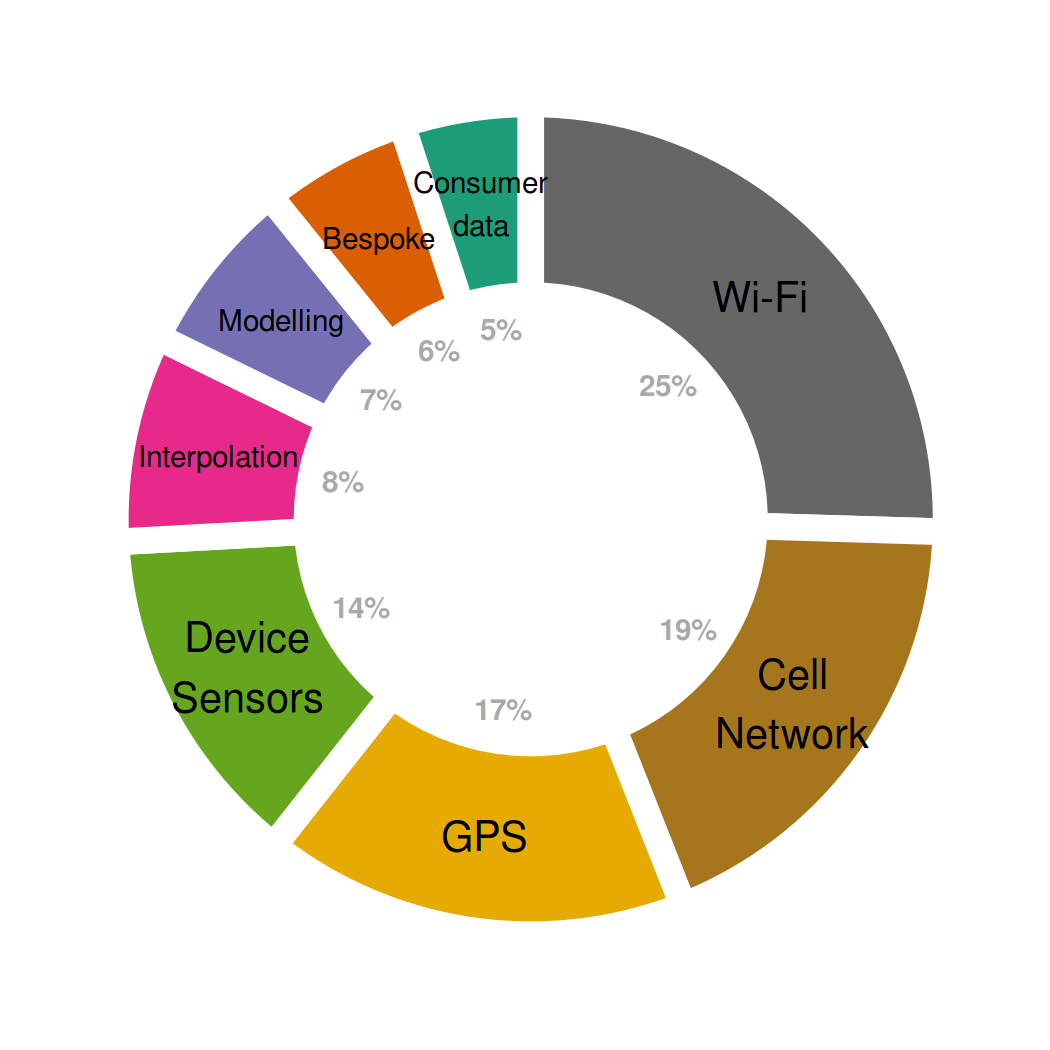
\includegraphics[trim={1.1cm 1cm 1cm 1cm},clip]{images/literature-technology.png}
  \caption{Distribution of research across various techniques and technologies}
  \label{figure:literature:timeline}
\end{marginfigure}
\marginnote{\noindent\fontsize{7}{7}\textit{Measured in the number of papers published}}

When we look at the literature from the technology perspective, we observe that over the years, the research continuously picks up and applies recent technological developments in the pursuit of understanding the distribution of human activity and population.
Figure \ref{figure:literature:timeline} shows the distribution of the research in terms of the main technique/ technology used over the past 40 years.
We observe that the earliest attempts started from the exploration of using interpolation and modelling techniques on a broader dataset.
As the need for more granular datasets increased there were attempts to devise and utilize bespoke solutions to generate them.
When mobile devices became mainstream, the focus shifted to utilize the relevant components of the mobile infrastructure.
A significant number of studies were done in utilising data collected from the mobile network, sensors in the mobile devices, especially GPS and Wi-Fi, in addition to the social media content generated from these devices.
A detailed account of these studies is given below,

\begin{figure*}
  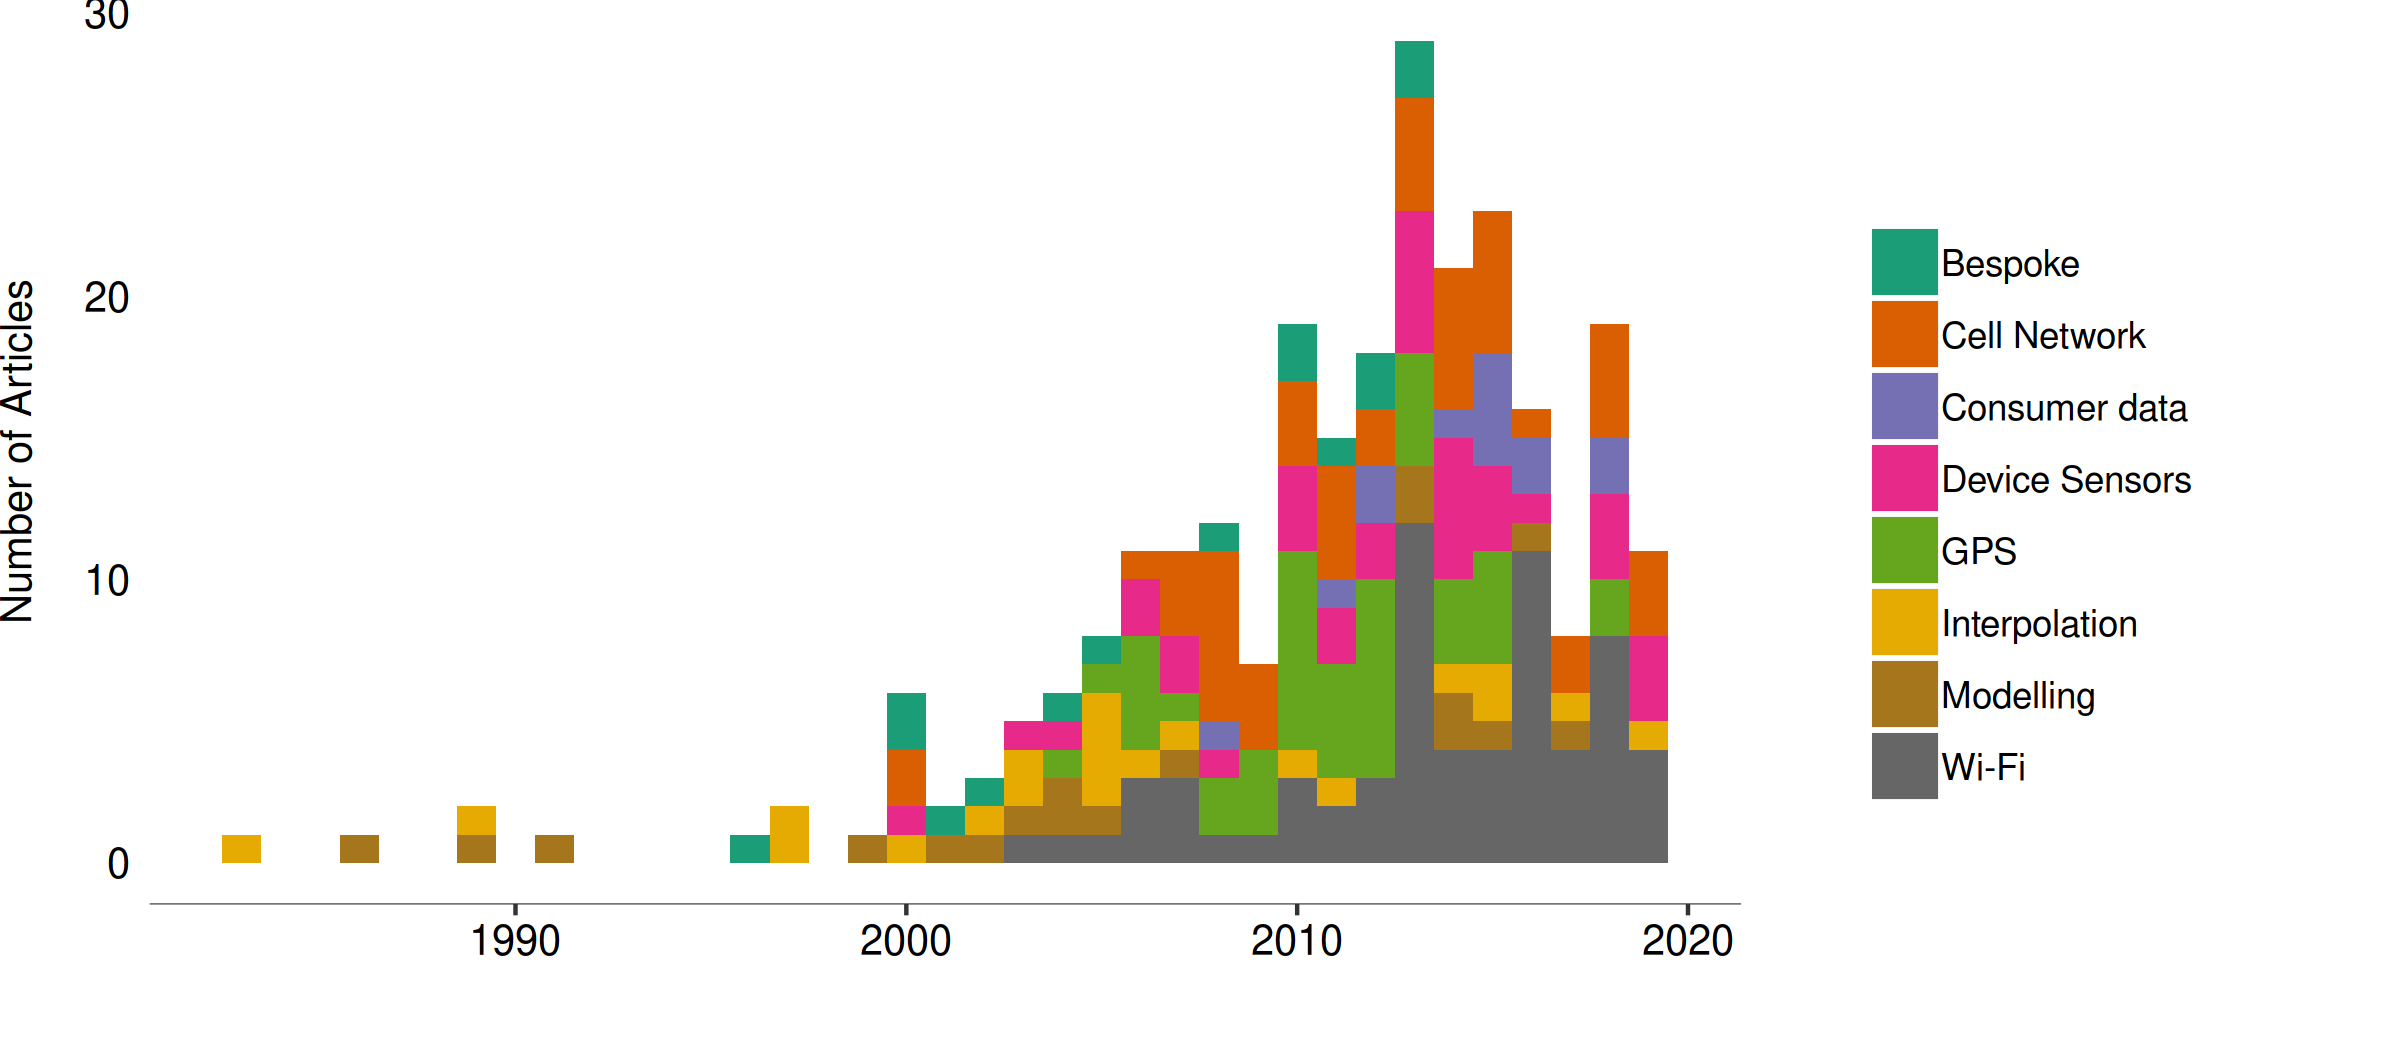
\includegraphics{images/literature-tech-timeline.png}
  \caption{The evolution of research since 1980 in terms of the the technology used in the research.}
  \label{figure:literature:tech:timeline}
\end{figure*}

%------------------------------------------------------------------------------%
\subsection{Interpolation and Modelling}
%------------------------------------------------------------------------------%

Attempts in using the existing data collected through traditional methods such as census and large scale sample surveys to create spatially and temporally granular and detailed estimates were carried out by applying various interpolation methods such as pycnophylactic, dasymetric interpolation \citep{tobler1979, mennis2003, mennis2006, hawley2005, tapp2010, wismans2017} along with spatial \citep{lam1983,martin1989, martin2015} and temporal interpolation techniques \citep{glickman1986}.
These methods along with supplementary data such as remote sensing imagery \citep{sutton2001, chen2002} and street networks \citep{reibel2005} were shown to be useful in producing detailed granular population maps at various scales with varying degree of success \citep{dobson2000, bhaduri2002, dobson2003, bhaduri2005, bhaduri2007}.
These approaches have been employed in various applications such as econometric studies \citep{mcdonald1989}, studies on public health \citep{hay2005}, emergency management \citep{kwan2005} and flood risk estimations \citep{smith2016}.

In addition to these interpolation techniques classic modelling techniques can also be used to estimate daytime populations and demographic structure at hyper-local scales \citep{jochem2013, jia2014}, urban scales \citep{alahmadi2013, abowd2004} and regional scales \citep{foley1954, schmitt1956, singleton2015, mccormack2017}.
The granular data created with such modelling techniques are shown to be useful in urban planning and management \citep{parrott1999}, emergency management \citep{alexander2002, cutter2006} and in modelling traffic and transportation \citep{lefebvre2013}.
These interpolation and modelling techniques along with granular data produced are also used in classifying spatial areas and hence understanding the structure of cities in general \citep{mcmillen2001, mcmillen2004, lee2007, arribas-bel2014}.
Though being useful, these techniques are still shown to have limitations and uncertainties \citep{nagle2014}, which mostly arise from the nature of the input data employed.
This leads us to the need for more detailed and frequent collection of data.

%------------------------------------------------------------------------------%
\subsection{Bespoke technologies}
%------------------------------------------------------------------------------%

Following this need, there has been efforts to use bespoke or specialised technologies such as cameras \citep{cai1996, heikkila2004, krockel2012}, Lasers \citep{zhao2005, arras2008} and radio frequency receivers  \citep{bahl2000, yang2013, chothia2010, bulusu2000, dil2011} to measure human activity.
But the major problem with such solutions is the cost and effort involved in designing and implementing them at urban and regional scales comprehensively.
Moreover, being specialised and centralised they tend to be challenging to maintain and update as the technological landscape change.
This gives us the need to identify and use techniques which are more general in nature and can be used for longer periods of time which are cheap to install to achieve a more comprehensive coverage.

%------------------------------------------------------------------------------%
\subsection{Cellular Network}
%------------------------------------------------------------------------------%

The rise of mobile phones as ubiquitous personal devices for the broader population has provided us with a viable alternative for collecting data with finer granularity at large scales.
Mobile infrastructure consists of both the `network part’, built and managed by the service providers, and the `user part’, which is the phones owned by the users’ themselves.
The network part, in addition to providing connectivity to the users, also collects information on these devices actively such as communication between the users and passively such as when the phones themselves move from tower to tower.
The mobile devices themselves have a variety of sensors such as accelerometer to identify movement, compass to identify orientation, GPS receiver to deduct geographic position, etc.
They also have various communication capabilities such as cellular, Wi-Fi, Bluetooth and Near field communications (NFC) etc. 
Both of these sensors and communication capabilities can be used as sources of data themselves.
With the growth of mobile devices and the infrastructure surrounding it, there has been significant effort in utilising data generated by every component of this complex infrastructure.

The first set of research started to use the cellular network data for urban studies \citep{jiang2013,steenbruggen2015, lokanathan2015, calabrese2015, reades2007}.
Even though this approach has been acknowledged to have inherent biases such as ownership bias across particular demographic groups \citep{wesolowski2013} the relative advantages such as coverage made them excellent sources of data.
Visual exploration of use of such data using interactive interfaces to evaluate quality of service and scenario testing has been tested for the optimisation of public transport \cite[-4cm]{sbodio2014}.
Such network data with the active and passive information collected from them can be used to create trajectories of people \cite{schlaich2010}, detect their daily routine \cite[2cm]{sevtsuk2010} and classify those routes in terms of function \citep{becker2011a}.
It was also demonstrated to be useful in understanding overall mobility and flow of people and information \citep{candia2008, krings2009, simini2012, zhang2019}.
These data can be used to identify asymmetry in flow of people spatially \citep{phithakkitnukoon2011}, estimate volume and pattern of road usage \citep{bolla2000, wang2012} and by augmenting the topology to optimise operations \citep{puzis2013}.
Such datasets have been extensively used in traffic and transportation research to derive origin-destination matrices \citep{caceres2007, mellegard2011, iqbal2014}, travel time estimation \citep{janecek2012} and traffic status estimation \citep{demissie2013, grauwin2015}. 

It has been shown that mobile network data can be used to uncover nature of the population such as tourists in specific areas \citep{girardin2008} and the interaction between the people in the study area \citep{campbell2008}.
The structure \citep{onnela2007, onnela2007a}, geography \citep{lambiotte2008} and dynamics \citep{hidalgo2008} of such networks have been studied and demonstrated to be useful in predicting their change \citep{wang2011, vajakas2018} over time.
This social networks and their spatio-temporal structure can also be used for classification of land use \citep{pei2014, jia2018}, assessment of spatial patterns \citep{reades2009, steenbruggen2013} and understanding the broader spatial structure of cities \citep{louail2014, arribas-bel2015} and regions \citep{arhipova2018}.
The data collected from the cellular network when examined at granular levels such as inter-personal communication and economic activity can be used to create estimations of micro area-level population density \cite[-6cm]{pulselli2008, ng2017} and also the characteristics \cite{girardin2009} and the nature of the activity \citep{phithakkitnukoon2010}.
Aggregated human activity measured from such research in turn can be used to measure and model population dynamics and land use density and mix at broader level \citep{jacobs-crisioni2014, tranos2015, tranos2018}.
The spatial patterns thus uncovered can then be applied to urban planning \citep{becker2011b} whilst the temporal patterns uncovered have immense utility for the disciplines such as epidemiology.
For example, population influxes measured from changes in mobile network usage can be used to model spread of diseases \cite{buckee2015}.

Though the mobile network provides much more granular and accurate data than interpolation techniques, it is not without its limitations \citep{yucel2017}.
The distribution of network infrastructure usually follows the purposes of service coverage and follows commercial decisions. 
This introduces systematic biases in the data passively collected through them.
Moreover, the data actively collected through them has bias based on the volume of usage of services by the customers which can vary widely spatially, temporally and also based on demography.
In addition to this because of the coverage, the data collected from mobile service providers pose immense privacy risk when linked to other sources of consumer data.
This makes collection of data directly from the devices using the sensors on the device much more robust in certain cases.

%------------------------------------------------------------------------------%
\subsection{Mobile Sensors}
%------------------------------------------------------------------------------%

The most prominent sensors and capabilities present in mobile devices that can be used for distributed urban sensing are Cellular radio, Bluetooth, Wi-Fi, GPS, accelerometer and compass \cite[-5cm]{lane2010, zhu2018}.
Since cellular radio is managed by the cellular network and covered in mobile network data, we explore the research done with other sensors.
In contrast to planned actively collected data, data passively collected via a distributed network of general purpose devices tends to be larger and more temporally dynamic.
For example, an organised survey conducted every month to understand interpersonal communications between people in a team of 50 will result in a 2500 records a month.
The same task is done through collecting data on email communication sent by them will result in a same volume records in a day.
The challenges and solutions on collecting and analysing such large-scale longitudinal data are discussed by \citep{laurila2012, antonic2013}.
The real time nature of such data also gives us the opportunity to monitor and understand the city in much smaller temporal scales \citep{townsend2000, oneill2006} and the representativeness of such datasets have also been explored \citep{shin2013, kobus2013}.
Data generated from communication networks can be used to understand the structure of urban systems which are becoming increasingly border-less \cite{bertolini2003}.
Similar to the network based data, it can help in understanding human mobility \citep{asgari2013, amini2014, zhang2014} through mining trajectory patterns \citep{giannotti2007} and socio geographic routines \citep{farrahi2010}.
It is also useful in various traffic and transportation applications for monitoring roads \citep{mohan2008} and estimating traffic \citep{cheng2006}, uncovering regional characteristics \citep{chi2014} and extracting land use patterns \citep{shimosaka2014}.
Apart from GPS and Wi-Fi, there have been efforts in exploring other possibilities such as Bluetooth for location \citep{bandara2004, becker2019} and aggregate detected Bluetooth activity to monitor freeway status \citep{haghani2010}.
There have also been successful implementations of frameworks to predict movement of people by combining Wi-Fi and Bluetooth \cite{vu2011}.
But owing to shorter range and requirement of active engagement from the user where they have to actively start the device pairing process, Bluetooth is much less preferable for large-scale data collection than GPS or Wi-Fi.
The research on GPS and Wi-Fi based studies are discussed in more detail below.

%------------------------------------------------------------------------------%
\subsection{Global Positioning System}
%------------------------------------------------------------------------------%

In addition to providing a user’s location to applications such as maps and navigation, the GPS capability in mobile devices in tandem with Wi-Fi can also maintain a continuous list of locations visited by the device over long periods of time.
It works mostly in the background and requires almost no active input from the user to operate.
Though very convenient for collecting data, due to the privacy risks associated with it, GPS is often one of the resources in a device that requires explicit user permission to be accessed.
The concepts and methodologies for collecting such data were set out by \citep{asakura2004} and there have been attempts to collect this rich data from volunteers at a large scale along with ancillary data \citep{kiukkonen2010} and provide a location based service application for the collection of data \citep{ratti2006, jiang2006, ahas2005}.
 
The accuracy, convenience and being designed for navigation makes GPS one of the most used technologies for mobility studies \cite{gonzalez2008}.
It has been used to analyse and understand individual mobility patterns \citep{neuhaus2009, shin2010}, which have been shown to have a high order of regularity in spite of the complexity \citep{brockmann2006, song2010a}.
There have been efforts to use this regularity to predict the future location of people \citep{monreale2009, calabrese2010}.
The limitations of predictions have also been quantified \citep{song2010}.
There have been successful efforts in extracting behaviours and patterns from such trajectory data \citep{liu2010, cho2011, hoteit2013, pappalardo2013} along to understand individual patterns from large assemblages \citep{giannotti2011, calabrese2013} and vice versa \citep{wirz2012}.
In traffic and transportation, GPS trajectory from mobile devices is used to estimate \citep{calabrese2011} and expand \citep{jing2011} origin-destination matrices, detect the mode of travel \citep{gong2012, rossi2015} and calibrate existing spatial interaction models \citep{yue2012}
.
Since the data is collected at the device level and depends on the activity of the individual, it can be de-anonymised to reveal the nature of the owner of the devices.
The possibilities of detecting the activity of the individual from trajectory information is demonstrated by \citep{liao2006, krumm2007}.
Patterns \citep{jiang2012} and structures in routines \citep{eagle2009} can be extracted from these trajectories and can be used for socio geographic analysis of the population \citep{licoppe2008, chen2018}.
It can also utilised in classification of the population at a particular location at a given time \cite[-1cm]{pappalardo2015}.
Being inherently spatial and activity driven, GPS trajectories have been shown to be useful to identify \citep{bao2012}, characterise \citep{wan2013} and automatically label \citep{do2014} significant places of interest.
It can also be used for land use detection \citep{toole2012, zhang2018}, classification \citep{jiang2015} and the study of urban morphology \citep{kang2012}.
These GPS trajectories have been shown to be useful in estimating population dynamics at local level and within short durations during social events \citep{calabrese2010, kim2014, deville2014}.
When combined with other data sources can be useful to understand relationship between spatial areas \citep{long2015}.

From the literature we see that GPS is one of the most precise and accurate user side methods of collecting location of mobile devices.
In addition, the data collected is well understood and collection methodologies can be scaled up with minimum resources.
That being said, it is also well established that urban sensing methods using GPS of mobile devices has problems of enhanced risk of breach of privacy when executed passively and need explicit user engagement when executed actively.

%------------------------------------------------------------------------------%
\subsection{Wi-Fi}
%------------------------------------------------------------------------------%

Wi-Fi is a wireless network connection protocol standardised by \citet{ieee2016}.
It is a distributed server-client based system where the client connects to access points (AP).
Every mobile device in the network has a unique hardware specific MAC address, which is transmitted between the device and AP before the connection is made.
The key feature of Wi-Fi infrastructure is that the network is distributed and the APs can be set up and operated by anyone locally unlike mobile networks.
Since they are primarily used for Internet service provision, the protocol has priority for continuity of connectivity so the devices constantly scan for new and better connections.
This is done through a probe request, which is detailed in later sections.
With this background we can see that Wi-Fi provides a fair middle ground between an entirely network driven approach such as cellular network to an entirely user driven approach such as GPS.
Since the network infrastructure is distributed and deployed for Internet it offers more coverage than most of the technologies discussed except or cellular network. It is also very resilient and can encapsulate and reinforce civic space in cities \cite{torrens2008}.

Though Wi-Fi is a location less technology, there are reliable methods to trilaterate the location of the device by the signal strength and the locations of APs known through either targeted surveys or crowdsourced volunteer effort \citep{he2003, moore2004, lamarca2005, dinesh2017, lin2018}.
This can overcome the usual shortcoming of GPS, which struggles for precision and accuracy in indoor and densely built environments \citep{zarim2006, kawaguchi2009, xi2010}.
Utilising this, we can easily and quickly estimate trajectories of the mobile devices just using the Wi-Fi communication the device has with multiple known APs \cite{xu2013}.
This can be used similar to the GPS trajectories to understand individual travel patterns \citep{kim2006, rekimoto2007, sap2015}, crowd behaviour \citep{abedi2013, mowafi2013, shu2017}, vehicular \citep{lu2010} and pedestrian movement \citep{xu2013, fukuzaki2014, wang2016, taylor2019}.
It can also be used in transportation planning and management to estimate travel time \citep{musa2011, haakegaard2018} and real time traffic monitoring \citep{abbott-jard2013}.

Being a general network protocol designed to be used by mobile devices, Wi-Fi devices relay a range of public signals known as probe request frames on regular intervals throughout its operation, for the purpose of connecting and maintaining a reliable and secure connection for the mobile device \cite{freud2015}.
These signals can be captured using inexpensive customised hardware, non-intrusively and in turn to be used for numerous applications.
In addition to a uniquely identifiable MAC address, these signals include a range of other information which when combined with the temporal signatures of the signals received can help us understand the nature and identify the devices which are generating these signals.
These device/user fingerprinting techniques are demonstrated by \citep{franklin2006} and \citep{pang2007} and the unique MAC addresses and associated information can successfully track people across access points \cite{cunche2014a}, their trajectories \citep{musa2012}, the relationship between them \citep{cheng2012, barbera2013, cunche2014} and predict which of them will be most likely to meet again \citep{cunche2012}.
Using the semantic information present in these probe requests, such as names of previously connected APs, it is possible to understand the nature of these users at a large scale \citep{di2016}.
Using the received signal strengths from pre placed devices we can monitor the presence and movement of entities that are not even carrying a Wi-Fi enabled device \cite{elgohary2013}.

Because of the security and privacy risks posed by the Wi-Fi protocol’s use of hardware based MAC address, various methods to strengthen the security have been proposed \citep{pang2007, greenstein2008}.
The randomisation of MAC addresses has become more mainstream in mobile devices with the introduction of it as a default operating system behaviour in iOS 8 by Apple Inc.
Since MAC randomisation is not a perfect solution \citep{mathieucunche2016} there have been numerous attempts to fingerprint unique devices from the randomised anonymous information present in the probe request frames for the purposes of trajectory tracking and access point security.
The methods used are decomposition of OUIs where detailed device model information is estimated by analysing an already known dataset of OUIs \cite{martin2016}; Scrambler attack where a small part of the physical layer specification for Wi-Fi is used \citep{bloessl2015}; and finally, the timing attack where the packet sequence information present in the probe request frame is used \citep{matte2016, cheng2016}.
A combination of these methodologies has been proven to de-anonymise randomised MAC addresses \citep{vanhoef2016}.
In addition to tracking, Wi-Fi probe requests can be aggregated to uncover the urban wireless landscape \citep{rose2010} and used to reveal human activity at large scales \citep{qin2013}, pedestrian numbers in crowds \citep{schauer2014, fukuzaki2015} and also counting people in hyper local scales such as queues \citep{wang2013}.
With enough infrastructure we can aim to generate a real-time census of the city \citep{kontokosta2016} and also predict the amount of time a device will spend around the sensor as well \citep{manweiler2013}.
Similar to GPS data this can be used as an additional control layer for interpolation techniques such as map merging \citep{erinc2013}.
A comparison of various approaches was done through experiments on a telecom operator dataset, where it was showed that using network-driven mobile phone location data is more advantageous compared to the widely used event-driven ones\cite[-3cm]{pinelli2015}.

%------------------------------------------------------------------------------%
\subsection{Consumer data}
%------------------------------------------------------------------------------%

In addition to the direct data from the sensors themselves the content generated from the mobile devices such as social media data or smart-cards \cite{zhong2016} can provide a viable proxy for estimating the level and nature of human activity.
The use of geo-located tweets on the study of small-area dynamic population estimation \citep{ordonez2012, marchetti2015, mckenzie2015, lansley2016a}, geo-demographics \citep{bawa-cavia2011, longley2015, lansley2016b} and global mobility \citep{hawelka2014} has been thoroughly explored.
These data sources are shown to be useful in social sciences \citep{crane2008}, abnormal event detection \citep{chae2012} and analysing urban environments \citep{sagl2012}.
It can also be used as a control layer for interpolation techniques we discussed earlier \citep{lin2015}.
